% AAAI-27 preliminary draft.
% Official AAAI-27 author-kit files exist at https://aaai.org/authorkit27/
% and include aaai2027.sty, aaai2027.bst, sample sources, and the
% reproducibility checklist. Place those files next to this draft before
% compiling in the official format.
\documentclass[letterpaper]{article}

% Enable once aaai2027.sty from the official author kit is in this directory.
% \usepackage[submission]{aaai2027}
\usepackage{times}
\usepackage{helvet}
\usepackage{courier}
\usepackage[hyphens]{url}
\usepackage{graphicx}
\usepackage{amsmath,amssymb}
\usepackage{booktabs}
\usepackage{multirow}
\usepackage{xcolor}

\title{From Feature Suppression to Feature Reliance: Diagnosing Shape, Texture, and Color Dependence under Natural Distribution Shift}

\author{
Anonymous Authors
}

\begin{document}
\maketitle

\begin{abstract}
Deep visual classifiers often fail under natural distribution shift, yet the
feature-level causes of such failures remain difficult to measure. A common
explanation is that ImageNet-trained models rely excessively on texture, but
recent controlled-suppression studies suggest that this picture is incomplete:
models may depend on color, texture, or shape in ways that vary across
architectures and domains. We present a diagnostic framework for measuring
\emph{feature reliance} by applying controlled image transformations that
selectively suppress color, texture, or shape while tracking accuracy,
representation similarity, and predictive distribution shift. We evaluate
ResNet-50 and ViT-B/16 on ImageNet, an ImageNet-200 subset aligned with
ImageNet-R, and ImageNet-R. Across 2,376 evaluation rows from 66 perturbation
settings, shape-disrupting transformations cause the largest reliance scores,
especially under ImageNet-R style shift, while texture suppression is often
less damaging than expected. ViT-B/16 is more stable than ResNet-50 under
moderate perturbations, but both models suffer severe failures under local
geometric warping. We further outline a sparse-autoencoder validation protocol
for testing whether hidden ViT features expose disentangled reliance factors.
These results support feature reliance as a practical lens for diagnosing
out-of-distribution robustness and for designing targeted data-centric
interventions.
\end{abstract}

\section{Introduction}

Modern image classifiers can achieve high in-distribution accuracy while
remaining brittle under domain shift. The brittleness is not only a property of
the final decision boundary: it often reflects which visual evidence the model
uses. If a classifier relies on fragile cues such as local texture, it may fail
when the same object appears in a different style or rendering. Conversely, if
it relies on shape cues, it may be more robust to some texture shifts but
sensitive to geometric disruption.

The long-standing ``texture bias'' hypothesis argues that ImageNet-trained CNNs
prefer local texture over global shape \cite{geirhos2019imagenet}. However,
recent work revisiting feature reliance through controlled suppression reports a
more nuanced story: measured reliance depends strongly on how visual attributes
are suppressed \cite{burgert2025feature}. This motivates a practical question
for robustness research: can we diagnose which feature families a model relies
on before designing out-of-distribution (OOD) interventions?

We study this question using controlled transformations that suppress or
perturb color, texture, and shape. Given an original image $x$ and transformed
image $\tilde{x}_f$ suppressing feature family $f$, we measure performance
degradation relative to chance-corrected original accuracy, together with
representation and output changes. Our experiments compare ResNet-50 and
ViT-B/16 on ImageNet, ImageNet-200, and ImageNet-R. The ImageNet-200 split uses
the ImageNet-R class subset, allowing us to compare in-distribution and natural
style-shifted evaluation over the same label space.

The empirical pattern is clear. Color removal is consistently mild. Texture
suppression through bilateral filtering is also moderate, and on ImageNet-R it
can be nearly neutral for ResNet-50. By contrast, shape-disrupting patch
shuffle, patch rotation, and local warping induce the largest failures,
particularly on ImageNet-R. The result is not that texture is irrelevant, but
that robustness failures cannot be explained by a one-dimensional texture-bias
story. Feature reliance must be measured along multiple axes.

Our contributions are:
\begin{itemize}
    \item We implement a controlled feature-reliance evaluation pipeline for
    color, texture, and shape perturbations across ImageNet, ImageNet-200, and
    ImageNet-R.
    \item We report architecture- and domain-specific reliance patterns for
    ResNet-50 and ViT-B/16 using accuracy, relative accuracy, Jensen-Shannon
    divergence, and centered kernel alignment (CKA).
    \item We introduce a sparse-autoencoder (SAE) validation protocol for
    connecting input-level suppression to latent feature factors in ViT
    activations.
\end{itemize}

\section{Related Work}

\paragraph{Texture and shape bias.}
Geirhos et al. showed that ImageNet-trained CNNs often classify images using
texture cues and that increasing shape bias can improve robustness
\cite{geirhos2019imagenet}. Follow-up work questioned whether texture bias is
an intrinsic property of ImageNet-trained CNNs or an artifact of how feature
reliance is probed \cite{burgert2025feature}. Our work follows the controlled
suppression perspective and extends it to natural style-shift evaluation.

\paragraph{Out-of-distribution generalization.}
OOD robustness benchmarks such as ImageNet-R evaluate whether classifiers
generalize from natural photographs to renditions, cartoons, paintings, and
other style-shifted images \cite{hendrycks2021many}. Domain generalization work
has also emphasized that simple data-centric interventions can be competitive
with more complex algorithmic changes \cite{gulrajani2021search}. We treat
feature reliance as a diagnostic step before choosing such interventions.

\paragraph{Representation similarity and mechanistic validation.}
CKA provides a stable measure of representation similarity across neural
networks and transformations \cite{kornblith2019similarity}. Sparse
autoencoders have recently become a common tool for discovering interpretable
latent directions in large models \cite{cunningham2024sparse}. In vision,
concept-level interpretability has been studied through unit-concept alignment,
open-world concept discovery, and sparse-autoencoder analysis of visual
representations \cite{bau2017network,kowal2024vcc,stevens2025saev}. Our SAE
validation protocol asks whether reliance factors measured at the image level
are reflected in sparse latent activations inside a ViT, and whether such
factors can ultimately support targeted representation-level control
\cite{flovik2025salve}.

\section{Method}

\subsection{Controlled Feature Suppression}

For each image $x$, we construct transformed images $\tilde{x}_f$ using
deterministic or stochastic transformations targeting a visual feature family
$f$:
\begin{itemize}
    \item \textbf{Color}: grayscale conversion with full color removal.
    \item \textbf{Texture}: bilateral filtering, which smooths local texture
    while preserving many edges.
    \item \textbf{Shape}: patch shuffle, patch rotation, and local geometric
    warping.
\end{itemize}

The implementation also records image-level suppression diagnostics: local
variance ratio (LV), high-frequency energy ratio (HFE), edge SSIM (ESSIM), and
gradient correlation (GC). Texture score is the mean of LV and HFE; shape score
is the mean of ESSIM and GC. Lower texture scores indicate stronger texture
suppression, while lower shape scores indicate stronger shape disruption.

\subsection{Feature Reliance Score}

Let $A_0$ be the model accuracy on original images, $A_f$ the accuracy after
suppressing feature family $f$, and $A_c = 1/C$ the chance accuracy for $C$
classes. We compute chance-corrected relative accuracy:
\begin{equation}
    R_f = \frac{A_f - A_c}{A_0 - A_c}.
\end{equation}
Feature reliance is then:
\begin{equation}
    \mathrm{FR}_f = 1 - R_f.
\end{equation}
A value near zero means the model remains accurate after suppressing $f$; a
value near one means the model collapses toward chance. We also compute
Jensen-Shannon divergence between original and transformed logits and linear CKA
between original and transformed representations.

\subsection{Sparse Autoencoder Validation}

To connect image-level reliance to latent features, we train a ReLU sparse
autoencoder on ViT-B/16 block activations. The current implementation collects
patch tokens from a target ViT block, normalizes token activations with
streaming statistics, initializes the decoder bias using a geometric median,
and trains an overcomplete dictionary with an L1 activation penalty:
\begin{equation}
    \mathcal{L}_{SAE}
    = \|x - \hat{x}\|_2^2 + \lambda \|z\|_1,
\end{equation}
where $z = \mathrm{ReLU}((x-b_{dec})W_{enc}+b_{enc})$ and
$\hat{x}=zW_{dec}+b_{dec}$. The validation script measures reconstruction MSE,
normalized MSE, cosine similarity, active latent counts, latent frequency, and
label entropy. In the next experimental iteration, we will compare SAE latent
activation shifts under each suppression family to test whether sparse factors
separate color-, texture-, and shape-sensitive concepts.

\section{Experimental Setup}

\paragraph{Models.}
We evaluate two pretrained models from \texttt{timm}: ResNet-50 with ImageNet-1K
weights and ViT-B/16 with augmented ImageNet-1K weights. Each model uses its
corresponding preprocessing statistics and resize/crop protocol.

\paragraph{Datasets.}
We evaluate on ImageNet validation, ImageNet-200, and ImageNet-R. ImageNet-200
is constructed by selecting the 200 ImageNet classes that overlap with
ImageNet-R. This allows direct comparison between in-distribution images and
natural OOD renditions with the same class space.

\paragraph{Perturbation sweep.}
We run 66 perturbation settings. Bilateral filtering sweeps sigma-color and
sigma-space values; local warping sweeps warp amplitude and smoothing; patch
shuffle and patch rotation use a fixed grid setting in the current result
table. Each setting evaluates original, grayscale, bilateral, patch shuffle,
patch rotation, and local warp variants. The resulting analysis table contains
2,376 evaluation rows.

\section{Results}

\subsection{Baseline Accuracy}

Table~\ref{tab:base} reports original-image accuracy. Both models perform
similarly on ImageNet and ImageNet-200, while ImageNet-R causes a large natural
OOD drop.

\begin{table}[t]
\centering
\small
\begin{tabular}{llr}
\toprule
Model & Dataset & Accuracy \\
\midrule
ResNet-50 & ImageNet & 0.8035 \\
ResNet-50 & ImageNet-200 & 0.9393 \\
ResNet-50 & ImageNet-R & 0.4021 \\
ViT-B/16 & ImageNet & 0.7914 \\
ViT-B/16 & ImageNet-200 & 0.9333 \\
ViT-B/16 & ImageNet-R & 0.3812 \\
\bottomrule
\end{tabular}
\caption{Original-image accuracy before controlled suppression.}
\label{tab:base}
\end{table}

\subsection{Feature Reliance Differs by Feature Family}

Table~\ref{tab:fr_mean} summarizes mean feature reliance across perturbation
settings. Color removal produces small reliance scores, with grayscale FR
ranging from 0.0577 to 0.1479. Bilateral texture suppression is also modest in
most settings and is nearly neutral for ResNet-50 on ImageNet-R. Shape
perturbations are substantially more damaging. On ImageNet-R, patch shuffle and
patch rotation produce FR above 0.60 for both models, and local warp reaches
0.7870 for ResNet-50 and 0.6314 for ViT-B/16.

\begin{table*}[t]
\centering
\small
\begin{tabular}{lllrrrrr}
\toprule
Model & Dataset & Perturbation & Acc. & Rel. Acc. & FR & CKA & JS \\
\midrule
ResNet-50 & ImageNet & Grayscale & 0.7271 & 0.9049 & 0.0951 & 0.7254 & 0.0947 \\
ResNet-50 & ImageNet & Bilateral & 0.6754 & 0.8404 & 0.1596 & 0.6756 & 0.1356 \\
ResNet-50 & ImageNet & Patch shuffle & 0.5087 & 0.6326 & 0.3674 & 0.4612 & 0.2709 \\
ResNet-50 & ImageNet & Patch rotation & 0.5005 & 0.6225 & 0.3775 & 0.4602 & 0.2790 \\
ResNet-50 & ImageNet & Local warp & 0.1856 & 0.2300 & 0.7700 & 0.3060 & 0.5261 \\
\midrule
ViT-B/16 & ImageNet & Grayscale & 0.6745 & 0.8521 & 0.1479 & 0.8363 & 0.1277 \\
ViT-B/16 & ImageNet & Bilateral & 0.6923 & 0.8746 & 0.1254 & 0.8768 & 0.1034 \\
ViT-B/16 & ImageNet & Patch shuffle & 0.5623 & 0.7102 & 0.2898 & 0.7933 & 0.2089 \\
ViT-B/16 & ImageNet & Patch rotation & 0.6004 & 0.7584 & 0.2416 & 0.8163 & 0.1770 \\
ViT-B/16 & ImageNet & Local warp & 0.3849 & 0.4857 & 0.5143 & 0.5793 & 0.3530 \\
\midrule
ResNet-50 & ImageNet-R & Grayscale & 0.3699 & 0.9190 & 0.0810 & 0.7722 & 0.1945 \\
ResNet-50 & ImageNet-R & Bilateral & 0.4029 & 1.0021 & -0.0021 & 0.7315 & 0.2213 \\
ResNet-50 & ImageNet-R & Patch shuffle & 0.1296 & 0.3137 & 0.6863 & 0.5189 & 0.4499 \\
ResNet-50 & ImageNet-R & Patch rotation & 0.1251 & 0.3024 & 0.6976 & 0.5415 & 0.4216 \\
ResNet-50 & ImageNet-R & Local warp & 0.0896 & 0.2130 & 0.7870 & 0.4433 & 0.4995 \\
\midrule
ViT-B/16 & ImageNet-R & Grayscale & 0.3418 & 0.8953 & 0.1047 & 0.7368 & 0.2081 \\
ViT-B/16 & ImageNet-R & Bilateral & 0.3709 & 0.9728 & 0.0272 & 0.7944 & 0.1639 \\
ViT-B/16 & ImageNet-R & Patch shuffle & 0.1376 & 0.3524 & 0.6476 & 0.5959 & 0.3399 \\
ViT-B/16 & ImageNet-R & Patch rotation & 0.1523 & 0.3916 & 0.6084 & 0.6495 & 0.2946 \\
ViT-B/16 & ImageNet-R & Local warp & 0.1436 & 0.3686 & 0.6314 & 0.5214 & 0.3554 \\
\bottomrule
\end{tabular}
\caption{Mean controlled-suppression results. FR denotes feature reliance
($1-\mathrm{relative\ accuracy}$); JS denotes Jensen-Shannon divergence.}
\label{tab:fr_mean}
\end{table*}

\begin{figure*}[t]
\centering
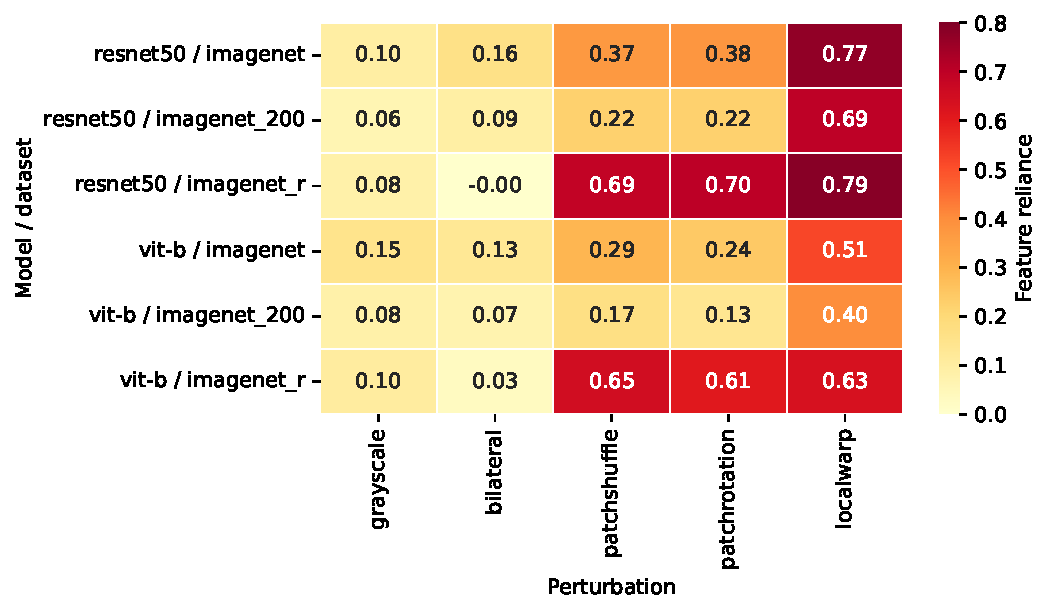
\includegraphics[width=0.92\textwidth]{figures/feature_reliance_heatmap.pdf}
\caption{Mean feature reliance across model, dataset, and perturbation family.
Shape-disrupting perturbations, especially local warp and patch-level
rearrangements, dominate the ImageNet-R failure pattern.}
\label{fig:fr_heatmap}
\end{figure*}

\subsection{Representation Shift Tracks Reliance}

Feature reliance correlates strongly with output and representation changes.
Across non-original evaluations, FR has correlation $0.9349$ with
Jensen-Shannon divergence and $-0.8188$ with CKA. Thus, perturbations that cause
accuracy collapse also induce larger predictive distribution shifts and lower
representation similarity. This supports the interpretation that feature
suppression affects internal representations, not merely final-layer calibration.

\begin{figure}[t]
\centering
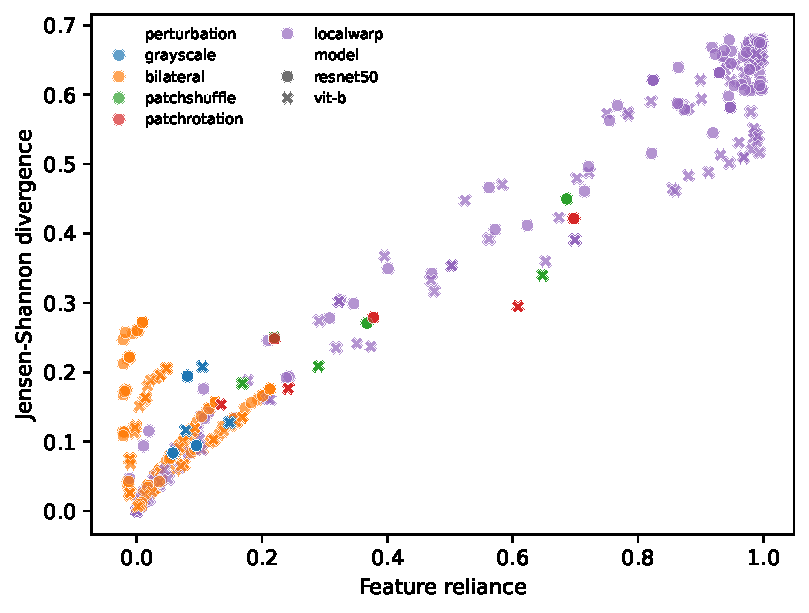
\includegraphics[width=\linewidth]{figures/fr_vs_js.pdf}
\caption{Feature reliance is strongly associated with predictive distribution
shift, measured by Jensen-Shannon divergence between original and transformed
logits.}
\label{fig:fr_js}
\end{figure}

\begin{figure}[t]
\centering
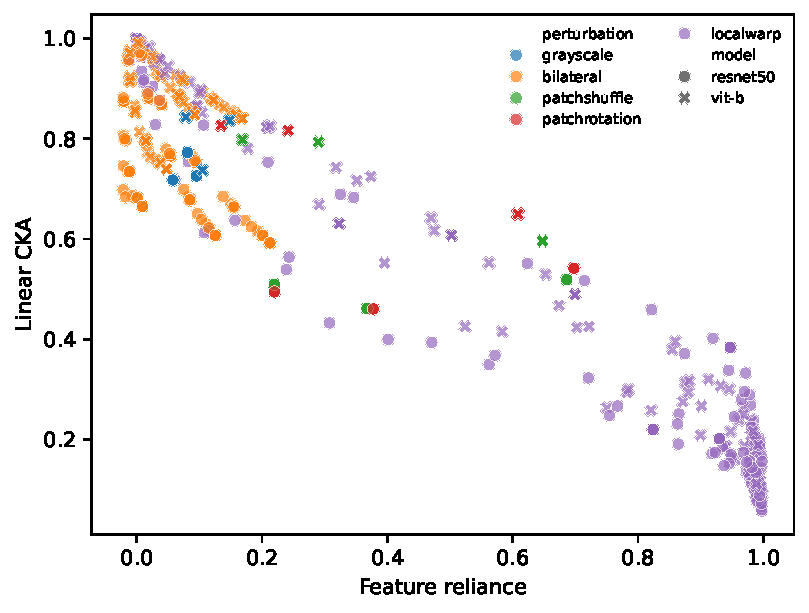
\includegraphics[width=\linewidth]{figures/fr_vs_cka.pdf}
\caption{Feature reliance is negatively associated with representation
similarity, measured by linear CKA between original and transformed
representations.}
\label{fig:fr_cka}
\end{figure}

\subsection{ViT-B/16 Is More Stable under Moderate Shape Disruption}

ViT-B/16 generally exhibits lower shape reliance than ResNet-50 on ImageNet and
ImageNet-200. On ImageNet, patch rotation gives FR $0.2416$ for ViT-B/16 versus
$0.3775$ for ResNet-50, and local warp gives FR $0.5143$ versus $0.7700$.
However, the advantage narrows under ImageNet-R: both architectures become
highly sensitive to patch-level shape disruption. This suggests that
architectural robustness is conditional on the domain and perturbation family.

\subsection{Severe Local Warping Exposes a Failure Mode}

The strongest local-warp settings collapse both models near chance. For example,
the best reliance setting on ImageNet uses alpha $80$ and sigma $0.5$, yielding
FR $0.9982$ for ResNet-50 and $0.9978$ for ViT-B/16. These results should not be
read as natural robustness estimates, because extreme local warp can produce
visually unnatural images. Instead, they expose a useful stress test: models
retain high-frequency texture statistics but fail when local geometry is
destroyed.

\section{Discussion}

The experiments challenge a simple texture-bias explanation for OOD failure.
Texture suppression is not uniformly catastrophic, and on ImageNet-R it can be
almost neutral. Shape disruption, by contrast, is consistently severe under
style shift. A practical implication is that robustness interventions should be
chosen based on measured reliance. If a model is already robust to texture
suppression but fragile to local geometry, adding more texture augmentation may
not address the dominant failure mode.

The SAE validation pipeline provides a route from diagnosis to intervention.
If sparse latent units show selective sensitivity to shape-preserving or
shape-disrupting transformations, then feature reliance can be studied not only
as an input-level phenomenon but also as a mechanistic property of hidden
representations. This opens the possibility of targeted latent editing,
regularization, or data augmentation guided by the discovered reliance factors.

\section{Limitations}

First, controlled suppression is only as valid as the transformation family.
Bilateral filtering, patch shuffling, and local warping are proxies for visual
feature removal, not perfect interventions. Second, the current experiments use
two pretrained architectures; broader claims require additional CNNs,
transformers, self-supervised models, and CLIP-like models. Third, local warp
contains extreme settings that are useful for stress testing but may not
represent natural distribution shift. Finally, the SAE component is currently a
validation protocol rather than a completed causal intervention; future work
should report latent-level perturbation and editing results.

\section{Conclusion}

We presented a feature-reliance diagnostic framework for measuring how visual
classifiers depend on color, texture, and shape under both in-distribution and
natural OOD evaluation. Across ResNet-50 and ViT-B/16, controlled suppression
shows that shape disruption is the dominant failure mode in our ImageNet-R
setting, while texture suppression is often less damaging than expected. These
findings suggest that feature reliance is a useful bridge between robustness
evaluation and targeted intervention design. The accompanying SAE protocol
points toward a mechanistic next step: identifying sparse latent factors that
explain and potentially control reliance under distribution shift.

\IfFileExists{aaai2027.bst}{\bibliographystyle{aaai2027}}{\bibliographystyle{plain}}
\bibliography{references}

\end{document}
